\part{Exercice 9}

\begin{itemize}
	\item[``$\implies$''] C'est du cours.
	\item[``$\impliedby$''] par contraposée : soit $G$ un supplémentaire de $F$ tel que $F \neq F^\perp$, et $p$ la projection sur $F$ parallèlement à $G$.

		Soit $u \in F \setminus \{0\}$, $v \in G \setminus \{0\}$ et \begin{align*}
			f: \R &\longrightarrow \R^+ \\
			\lambda &\longmapsto \|u + \lambda v\|^2 - \|u\|^2\\
			&\phantom{\longmapsto} = 2\lambda \left<u  \mid v \right> + \lambda^2 \|v\|^2
			&\phantom{\longmapsto} = \lambda (2\left<u \mid v \right> + \lambda \|v\|^2)
		\end{align*}

		\begin{center}
			\begin{tikzpicture}
				\tkzTabInit{$\lambda$/1,$f$/1}{$-\infty$, $0$, $\lambda_0$, +$\infty$}
				\tkzTabLine{,+,z,-,z,+,}
			\end{tikzpicture}

			ou

			\begin{tikzpicture}
				\tkzTabInit{$\lambda$/1,$f$/1}{$-\infty$, $\lambda_0$, $0$, +$\infty$}
				\tkzTabLine{,+,z,-,z,+,}
			\end{tikzpicture}
		\end{center}

		\[
			\forall \mu \in [0, \lambda_0],\,f(\mu) =  \|\underbrace{u + \mu v}_{x}\| - \|\underbrace{u}_{p(x)}\| < 0
		\] donc $\|x\| < \|p(x)\|$
\end{itemize}
